\documentclass{vhdl-assignment}

\title{Assignment 6}
\date{2023}

\begin{document}
\maketitle
\thispagestyle{fancy}

\begin{problem}{Use data flow model, screenshot desgin code, testbench code, waveform, code coverage report}
    \subsection*{1. Design circuits two numbers 4-bit}
    \begin{verbatim}
        Input : [3:0]A, B
        Output : 
        A_lt_B = 1 if A < B.
        A_eq_B = 1 if A = B.
        A_gt_B = 1 if A > B.
    \end{verbatim}

    \subsection*{2. Design and compare 4 – bit Full Adder with Carry Look Ahead Adder 4 – bit about: Structure, delay, speed}
    \begin{figure}[H]
        \centering
        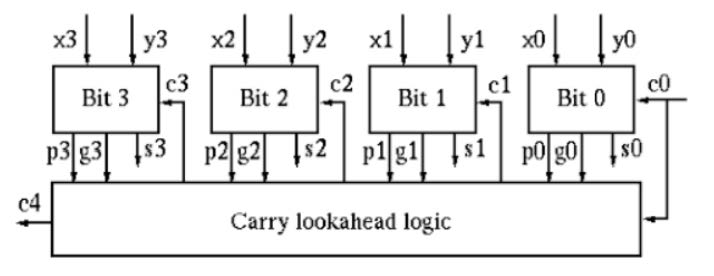
\includegraphics{assets/CarryLookAheadAdder.jpg}
    \end{figure}
\end{problem}

\begin{problem}{Answer the following questions}
    \begin{enumerate}
        \item Describe the statement assign (continuous assignment).
        \item Define, give examples of expressions, operands, operator in DataFlow Modeling.
        \item List the types of operators used in DataFlow Modeling (arithmetic, logical, relational, equality, bitwise, reduction, shift, concatenation, and conditional), give examples.
        \item Instruction: 6.1 Continuous Assignments,6.3 Expressions , Operators, and Operands, 6.4 Operator Types–Chapter 6. Dataflow Modeling–Verilog HDL Samir
    \end{enumerate}
\end{problem}

\end{document}